\documentclass[12pt,a4paper]{article}
\usepackage[T1]{fontenc}     
\usepackage[utf8]{inputenc}  % Accents codés dans la fonte
\usepackage[frenchb]{babel}  % Les traductions françaises
\usepackage{numprint}        % \numprint(9,36) pour utilisation de la virgule comme séparateur décimal

\usepackage{moreverb}

\usepackage{pdfpages}
\usepackage{hyperref}
\usepackage{multicol}
\setlength{\columnseprule}{1pt}
\usepackage{setspace}



\renewcommand{\baselinestretch}{1.3}
\usepackage[top=2cm, bottom=2cm, left=2cm, right=2cm]{geometry}

\usepackage{amsmath}         % Les maths de base

%\usepackage[svgnames]{xcolor}% Pour les besoins de PythonTeX
\usepackage{geometry}        % Gestion des dimensions des pages

\usepackage{tgpagella}       % Pour changer un peu les fontes
\usepackage{tgadventor}
\usepackage{inconsolata}

%\usepackage{minted}
\usepackage{pythontex}       % Utilisation de PythonTeX

\usepackage{graphicx}        % Gestion des inclusions
\usepackage{wrapfig}

\usepackage{tikz}            % Si on veut présenter le code Python
\usepackage[framemethod=TikZ]{mdframed}

\usepackage[colorinlistoftodos]{todonotes}
% Un environnement pour faire joli pour présenter le code Python
\newenvironment{code}{%
\begin{mdframed}[linecolor=Green,innerrightmargin=30pt,innerleftmargin=30pt,
backgroundcolor=Black!5,
skipabove=10pt,skipbelow=10pt,roundcorner=5pt,
splitbottomskip=6pt,splittopskip=12pt]
}{%
\end{mdframed}
}

% Un raccourci pour composer les unités en caractères droits
\newcommand{\U}[1]{~\mathrm{#1}}

% Présentation de l'abstract pour la problématique
\usepackage[runin]{abstract}

% Un environnement pour la problématique
\newenvironment{problematique}{
\renewcommand{\abstractname}{Problématique}
\begin{abstract}
}{
\end{abstract}
}


% Titre et auteurs du document
\title{Petit tuto \emph{git}}
\author{Charles VAN GOETHEM}
\date{}

% Et début du document proprement dit
\begin{document}

\maketitle

{\setstretch{1.1}
\begin{problematique}
Ici le but est d'apprendre à maîtriser la solution \emph{git} pour le développement de Nenufaar. L'objectif principal est de comprendre comment fonctionne \emph{git} et son utilité pour un développement collaboratif. Dans un premier temps, nous allons expliquer qu'est-ce que \emph{git} puis nous prendrons un exemple de développement.
% * <charles.van.goethem@gmail.com> 2017-01-09T11:18:09.001Z:
%
% ^.
\end{problematique}
}

\section{\emph{git} : kézako ?}

\subsection{Comment on gère un projet ?}

Avant d'utiliser un gestionnaire de versions, tu te dis que tu peux très bien gérer tes versions tout seul. Tu t'organises et décides de nommer tes fichiers avec leurs versions respectives. Puis tu crées des archives contenant chacune des versions de productions. Pour quoi apprendre à utiliser un logiciel pour faire ça ?

\begin{center}
% Inclusion d'une image: ce qui est entre crochets est un argument "optionnel", alors que l'argument obligatoire est entre accolades
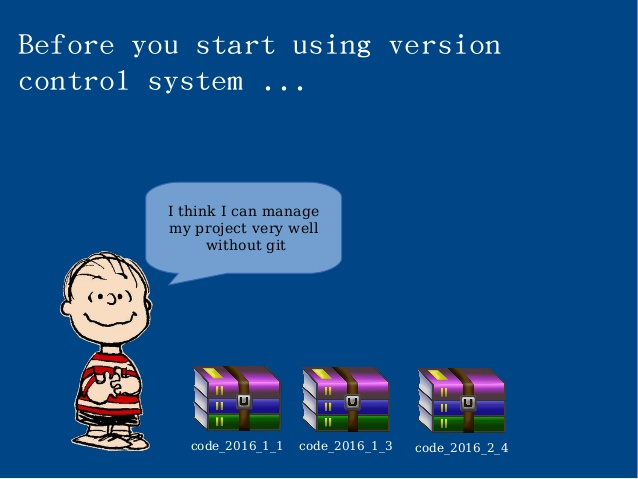
\includegraphics[width=.5\linewidth]{before_git}
\end{center}

Puis tu continues de développer et tu crées de plus en plus de versions. C'est cool jusqu'à ce qu'un collègue arrive et nous demande la version \emph{"tu sais avec la fonction qui faisait le truc là... C'était mieux !"} et que tu recherches la bonne version...

\begin{center}
% Inclusion d'une image: ce qui est entre crochets est un argument "optionnel", alors que l'argument obligatoire est entre accolades
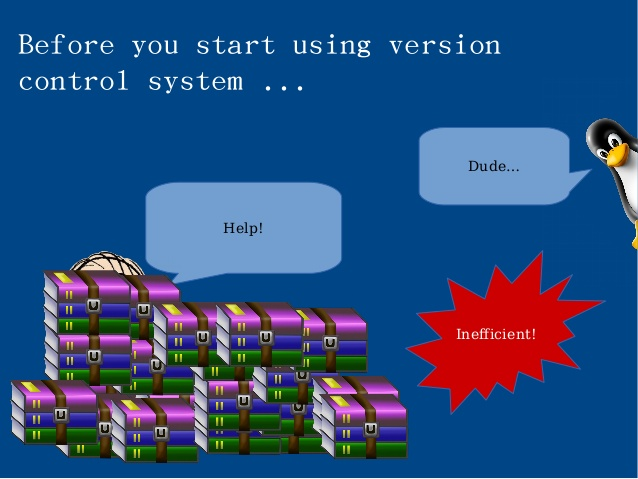
\includegraphics[width=.5\linewidth]{before_lost}
\end{center}

Maintenant, tu sais pourquoi on a besoin d'un gestionnaire de versions !

\subsection{Les gestionnaires de versions}

% Inclusion d'une image: ce qui est entre crochets est un argument "optionnel", alors que l'argument obligatoire est entre accolades
\begin{wrapfigure}{r}{0.3\linewidth}
\vspace*{-2.6\baselineskip}

\includegraphics[width=\linewidth]{yoda_git}
\end{wrapfigure}
On s'organise un peu et on va voir le vieux sage du coin. Il nous explique alors qu'à son époque, on savait coder et que l'on utilisait \emph{sccs} pour gérer les versions. Il t'explique que \emph{sccs} signifie \emph{Source Code Control System} et permet de gérer les versions d'un programme ! C'est ce que tu veux, mais c'est un peu vieux (1972) et puis c'est qu'en local... Le vieux sage t'explique alors qu'il existe des logiciels plus récents tels que \emph{subversion}, développé à la fin des années 90 et reposant sur le principe de développement centralisé, ou \emph{git}, développé au milieu des années 2000 et permettant de travailler de manière décentralisée. \emph{git} est parmi les plus répandus aujourd'hui avec plus de 12 millions d'utilisateurs et en plus c'est libre !

\emph{"La route est longue mais la voie est libre..."} --- \emph{\href{https://framasoft.org/}{framasoft.org}}

Pour résumer, un gestionnaire de version est donc un outil qui va permettre d'enregistrer les évolutions d'un projet au cours du temps. Et il existe 3 systèmes différents :
\begin{itemize}
\item[$\bullet$] local : très bien quand on travaille seul (\emph{sccs} -- 1972) 
\item[$\bullet$] centralisé : chacun travaille sur la version qu'il veut (\emph{subversion} -- 1998)
\item[$\bullet$] décentralisé : tout le monde peut disposer de toutes les versions (\emph{git} -- 2005)
\end{itemize}

\begin{center}
% Inclusion d'une image: ce qui est entre crochets est un argument "optionnel", alors que l'argument obligatoire est entre accolades
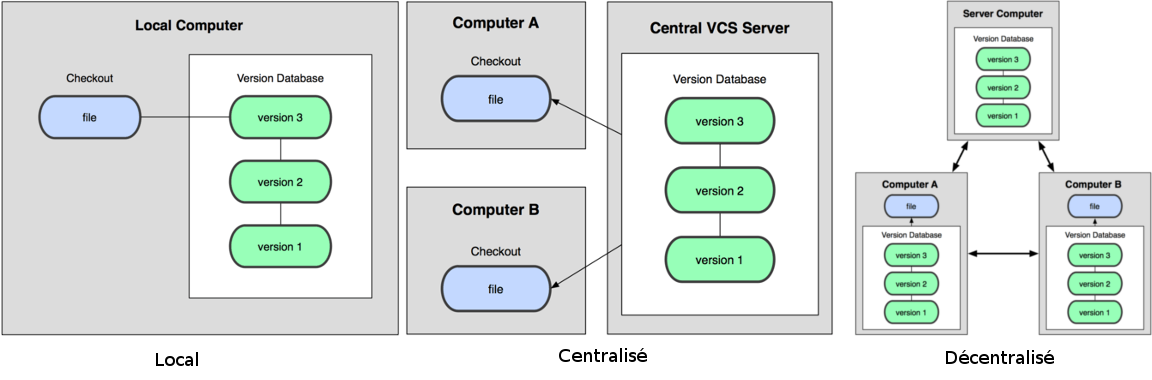
\includegraphics[width=0.9\linewidth]{gest}
\end{center}



\section{La base de \emph{git}}

% \begin{wrapfigure}{l}{0.3\linewidth}
% \vspace*{-1.\baselineskip}
% 
\includegraphics[width=\linewidth]{git_not_simple}
% \end{wrapfigure}
\begin{wrapfigure}[4]{r}{0.25\linewidth}
\vspace*{-1.2\baselineskip}
\centering

\includegraphics[width=\linewidth]{git_not_simple}
\end{wrapfigure}
\emph{"Apprendre git, ce n'est pas si simple"} --- Boromir, fils de Denethor.

Mais en vérité utiliser \emph{git} c'est comme tout ça s'apprend. Ce petit guide va permettre d'utiliser la base de \emph{git} mais il restera encore beaucoup à apprendre si vous le souhaitez !

\subsection{Utiliser \emph{git}}

\subsubsection{Configurer \emph{git}}

\emph{git} nécessite d'être configuré avant utilisation. Dans un premier temps, on doit préciser à \emph{git} qui on est et avec quel éditeur de texte tu préfères l'utiliser :

{
\setstretch{1}
\begin{boxedverbatim}
$ git config --global user.name "Foo Bar"
$ git config --global user.email foo.bar@example.com
$ git config --global core.editor vim
\end{boxedverbatim}
}

Là c'est cool \emph{git} sait qui tu es et avec quel outil tu souhaites travailler. On ne sait jamais vérifions que \emph{git} sache bien qui on est :

{\setstretch{1}
\begin{boxedverbatim}
$ git config user.name
Foo Bar
\end{boxedverbatim}
}

On peut donc vérifier une par une les infos ou alors toutes d'un coup avec la commande suivante :

{\setstretch{1}
\begin{boxedverbatim}
$ git config --list
user.name=Foo Bar
user.email=foo.bar@example.com
color.diff=auto
color.status=auto
color.branch=auto
push.default=matching
core.editor=vim
\end{boxedverbatim}
}

\subsubsection{Initialiser un projet}

Bon, maintenant on va voir comment créer un nouveau projet. Sans \emph{git} c'est facile, on crée un nouveau répertoire :

{\setstretch{1}
\begin{boxedverbatim}
$ mkdir Unicorn_project
\end{boxedverbatim}
}

Et avec \emph{git} pas d'affolement, c'est très simple aussi. On utilise \emph{git} pour initialiser notre projet :

{\setstretch{1}
\begin{boxedverbatim}
$ git init Unicorn_project
\end{boxedverbatim}
}

Félicitation, dans les deux cas, vous avez créé votre premier projet ! Par contre, on est en droit de se poser la question : \emph{Pourquoi, diable faire comme cela ?}

Et bien en utilisant la commande \emph{git init} on crée également le répertoire \emph{.git}. Ce répertoire contient toutes les infos dont \emph{git} a besoin pour gérer les versions.

\subsubsection{Travailler}

C'est bien beau tout ça, mais il faut travailler maintenant. Pour apprendre les bases de \emph{git} on va supposer que l'on travaille seul.

Alors, imaginons que l'on crée un super code :

{\setstretch{1}
\begin{boxedverbatim}
$ vi my_awesome_script.pl
$ more my_awesome_script.pl
#/usr/bin/perl

print "My little pony !\n";
\end{boxedverbatim}
}

Voilà notre premier script du projet fini ! On peut utiliser la commande suivante pour voir l'avancement du projet.
%\todo[inline, color=green!40]{Quelle commande ?}

{\setstretch{1}
\begin{boxedverbatim}
$ git status
Sur la branche master

Validation initiale

Fichiers non suivis:
  (utilisez "git add <fichier>..." pour inclure dans ce qui sera validé)

	my_awesome_script.pl

aucune modification ajoutée à la validation mais des fichiers non suivis sont
présents (utilisez "git add" pour les suivre)
\end{boxedverbatim}
}

Là \emph{git} nous signale que l'on a un fichier qui n'est pas \emph{"suivi"}. Cela signifie que ce fichier n'est pas encore enregistré par \emph{git}. Il faut donc préciser à \emph{git} que l'on utilise ce fichier (on verra plus tard comment ignorer certains fichiers), et on vérifie :

{\setstretch{1}
\begin{boxedverbatim}
$ git add my_awesome_script.pl 
$ git status
Sur la branche master

Validation initiale

Modifications qui seront validées :
  (utilisez "git rm --cached <fichier>..." pour désindexer)

	nouveau fichier: my_awesome_script.pl
\end{boxedverbatim}
}

Bon et maintenant il faut \emph{"commiter"} ses actions. \emph{"Commiter"} son code signifie soumettre, archiver son code. En même temps que l'on \emph{commit} le code on doit ajouter un message qui définit la modification effectuée. Traditionnellement le message "Initial commit" est associé au premier \emph{commit}.

{\setstretch{1}
\begin{boxedverbatim}
$ git commit -m "Initial commit"
[master (commit racine) e023001] Initial commit
 1 file changed, 3 insertions(+)
 create mode 100644 my_awesome_script.pl
$ git status
Sur la branche master
rien à valider, la copie de travail est propre
\end{boxedverbatim}
}

Bon, ben déjà avec ces quelques commandes on peut archiver nos projets de façon propre. C'est pas mal pour un début !


\subsubsection{Ignorer des fichiers}

\begin{wrapfigure}[8]{l}{0.3\linewidth}
\vspace*{-0.6\baselineskip}

\includegraphics[width=\linewidth]{dontcare}
\end{wrapfigure}

Bon alors, c'est déjà pas mal ! Maintenant, on va apprendre à ignorer des fichiers. En effet, dans un grand nombre de projets on génère des fichiers qu'il n'est pas utile d'archiver (notamment des fichiers temporaires, des logs...).

C'est pourquoi on peut indiquer à \emph{git} que certains de nos fichiers ne sont pas à prendre en compte. Ici on va voir deux exemples : un répertoire contenant les logs et des fichiers \emph{.bak} générés par un éditeur.

{\setstretch{1}
\begin{boxedverbatim}
$ git status
Sur la branche master
Fichiers non suivis:
  (utilisez "git add <fichier>..." pour inclure dans ce qui sera validé)
	PinkUnicornOfLove.sh
	PinkUnicornOfLove.sh.bak
	log/

aucune modification ajoutée à la validation mais des fichiers non suivis sont
présents (utilisez "git add" pour les suivre)
\end{boxedverbatim}
}

On a ici un script (\emph{PinkUnicornOfLove.sh}),  un fichier temporaire (\emph{PinkUnicornOfLove.sh.bak}) et un répertoire de log. Pour ignorer ces fichiers et répertoires, on va créer un fichier particulier :

{\setstretch{1}
\begin{boxedverbatim}
$ vi .gitignore
$ more .gitignore 
*.bak
log/
$ git status
Sur la branche master
Fichiers non suivis:
  (utilisez "git add <fichier>..." pour inclure dans ce qui sera validé)
	.gitignore
	PinkUnicornOfLove.sh

aucune modification ajoutée à la validation mais des fichiers non suivis sont
présents (utilisez "git add" pour les suivre)
\end{boxedverbatim}
}

\begin{minipage}{0.25\linewidth}

\includegraphics[width=\linewidth]{simple}
\end{minipage}\hfill
\begin{minipage}{0.7\linewidth}

Si l'on compare le résultat du \emph{git status} après création du fichier \emph{.gitignore} avec le précédent, on s'aperçoit que les fichiers se terminant par \emph{.bak} et le répertoire \emph{log/} ne sont plus pris en compte dans \emph{git}. Effectivement, ils n'apparaissent plus dans la liste des fichiers non-suivis.
% On voit qu'une fois le fichier \emph{.gitignore} créé le fichier \emph{.bak} et le répertoire \emph{log} ne sont plus sur la liste des fichiers non-suivis.
% \todo[inline, color=green!40]{Pas clair au dessus}


Et voilà, on sait maintenant utiliser \emph{git}. Au moins pour gérer de petits projets.
\end{minipage}

\subsection{Travailler à plusieurs}

Maintenant, on va compliquer un peu les choses avec le travail à plusieurs, mais en vérité c'est pas beaucoup plus complexe (en tout cas pour le début).

\subsubsection{cloner un dépôt}
% \todo[inline, color=green!40]{on comprend pas bien ou on veux en venir avec le clone il faudrait peut etre rajouter une phrase du style : pour qu'une personne se rajoute a un projet déjà existant, il faut qu'il puisse faire une copie de ce projet déjà existant. Pour cela on utilise la commande 'clone'}
Dans un premier temps, on va apprendre à cloner un dépôt déjà existant. Cela veut dire que l'on va créer une copie exacte du premier projet. Le clone va notamment permettre d'avoir sa propre copie du projet en local. On verra ensuite comment mettre à jour sa copie et envoyer ses propres modifications. Les deux copies auront donc le même historique et sont donc toutes les deux autant légitimes l'une que l'autre.

{\setstretch{1}
\begin{boxedverbatim}
$ git clone Path/project_A Path/project_b
Clonage dans 'project_b'...
remote: Counting objects: 14, done.
remote: Compressing objects: 100% (11/11), done.
remote: Total 14 (delta 5), reused 0 (delta 0)
Réception d'objets: 100% (14/14), 5.09 KiB | 0 bytes/s, fait.
Résolution des deltas: 100% (5/5), fait.
Vérification de la connectivité... fait.
\end{boxedverbatim}
}

\subsubsection{Maintenir à jour sa copie}

On va partir de l'hypothèse que le dépôt \emph{project\_A} est la référence et que le dépôt \emph{project\_b} est la copie locale. On suppose que des modifications sont apportés au dépôt A sans que vous ayez modifié le dépôt B.

Lorsque vous ferez un \emph{git status} dans le dépôt B, vous ne verrez pas de modification. En effet, il est à jour avec lui-même, il faut tester si le dépôt B est à jour avec le dépôt A.

{\setstretch{1}
\begin{boxedverbatim}
$ git status
Sur la branche master
Votre branche est à jour avec 'origin/master'.
rien à valider, la copie de travail est propre
$ git remote update
Récupération de origin
remote: Counting objects: 3, done.
remote: Compressing objects: 100% (3/3), done.
remote: Total 3 (delta 1), reused 1 (delta 0), pack-reused 0
Dépaquetage des objets: 100% (3/3), fait.
Depuis Path/project_A
   69e3c98..1bb5353  master     -> origin/master
$ git status
Sur la branche master
Votre branche est en retard sur 'origin/master' de 1 commit, et peut être mise
à jour en avance rapide.
  (utilisez "git pull" pour mettre à jour votre branche locale)
rien à valider, la copie de travail est propre
\end{boxedverbatim}
}

\emph{git} nous signale que nous ne sommes plus à jour par rapport au dépôt A. Il nous précise de faire un \emph{git pull}. Cette commande permet de récupérer les modifications sur le dépôt A.

{\setstretch{1}
\begin{boxedverbatim}
$ git pull
Mise à jour 69e3c98..1bb5353
Fast-forward
 README.md | 2 +-
 1 file changed, 1 insertion(+), 1 deletion(-)
\end{boxedverbatim}
}

On voit que l'on a récupéré deux modification sur le fichier README.md.

\subsubsection{Envoyer ses modifications}

Maintenant que l'on sait maintenir à jour un dépôt, on va voir comment envoyer ses modifications. Là aussi c'est simple une commande permet de le faire :

{\setstretch{1}
\begin{boxedverbatim}
$ vim README.md 
$ git commit -m "little"
[master 26074e3] little
 1 file changed, 1 insertion(+), 1 deletion(-)
$ git push
Décompte des objets: 3, fait.
Delta compression using up to 8 threads.
Compression des objets: 100% (3/3), fait.
Écriture des objets: 100% (3/3), 364 bytes | 0 bytes/s, fait.
Total 3 (delta 1), reused 0 (delta 0)
remote: Resolving deltas: 100% (1/1), completed with 1 local objects.
To https://github.com/...../
   1bb5353..26074e3  master -> master
\end{boxedverbatim}
}

Et voilà la modification est envoyée ! C'est ultra-simple non ? Bon alors évidemment là on suppose que l'on a bien fait un pull juste avant de modifier notre programme et que personne ne l'a modifié au même endroit... Pour bien comprendre la suite il faut savoir que la commande \emph{git push} est un alias de \emph{git push origin master} ce qui signifie que l'on envoi vers le lien d'origine (\emph{git remote -v}) sur la branche \emph{master}.

\subsubsection{La théorie des branches}

\begin{minipage}{0.7\linewidth}
Les branches sont très importantes sous \emph{git}. On verra dans la section suivante avec un exemple concret sur Nenufaar, comment on pourra les utiliser.
\end{minipage}\hfill
\begin{minipage}{0.25\linewidth}

\includegraphics[width=\linewidth]{branch}
\end{minipage}

Pour faire simple les branches sont des copies d'une autre branche (la première et principale est la branche \emph{master}). On va notamment souvent trouver une branche stable qui servira aux versions des projets (la branche de production, souvent \emph{master}) et une seconde branche qui servira a stocker les avancer régulière entre deux points stables (la branche de développement). Mais on va également pouvoir avoir un ensemble d'autres branches qui seront des corrections de bugs par exemple.

\centerline{
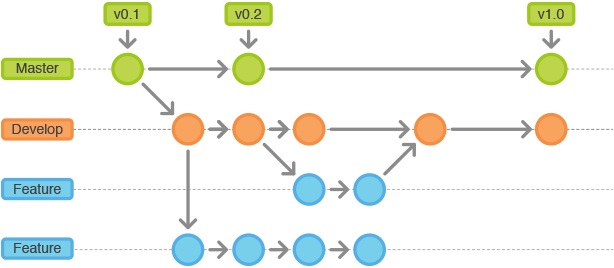
\includegraphics[width=0.7\linewidth]{git-branch}}

Sur ce graphique, on distingue 3 points stables de versions (en vert) sur la branche \emph{master}. Ensuite, on trouve une branche de développement (en orange), puis des branches concernant les features, ajout de nouvelles fonctions au programme (en bleu). La philosophie des auteurs, pour ce cas, est :
\begin{itemize}
\item[$\bullet$] pas de commit sur les branches \emph{master} et \emph{dev} ;
\item[$\bullet$] une branche par feature ;
\item[$\bullet$] les \emph{features} sont fusionnées sur la branche \emph{dev}.
\end{itemize}

Je ne vais pas aller beaucoup plus loin sur les branches puisque je l'expliquerais à l'aide d'un exemple concret plus tard. Je vais quand même expliquer les quelques commandes utiles pour leur manipulation.

Les commandes suivantes servent à créer, rejoindre, fusionner et supprimer des branches. Il faut également penser à envoyer ses modifications sur la branche spécifiée.

{\setstretch{1}
\begin{boxedverbatim}
$ git branch MyBranch		### créer la branche MyBranch
$ git checkout MyBranch		### rejoindre la branche Mybranch
$ git checkout -b MyBranch	### créer et rejoindre la branche Mybranch
$ git merge MyBranch		### fusionner la branch MyBranch avec la
branche courante
$ git branch -d Mybranch	### supprimer la branche MyBranch
$ git push origin Mybranch	### envoyer sur la branche MyBranch
\end{boxedverbatim}
}

\subsubsection{Résolution de conflits}

\begin{wrapfigure}{l}{0.28\linewidth}
\vspace*{-0.5\baselineskip}

\includegraphics[width=\linewidth]{gitmerge}
\end{wrapfigure}
Bon la théorie, c'est bien mais je tiens à vous le dire maintenant : vous aurez des erreurs ! C'est inévitable à force d'utiliser \emph{git} on se retrouvera avec des conflits de versions. Mais avant de paniquer, on va voir ce que c'est et apprendre à les gérer.

Déjà un conflit interviendra majoritairement au moment de la fusion de deux branches (\emph{git merge}). On pourra avoir des conflits si deux personnes ont travaillés ensemble sur le même point (même fichier, même zone).


% \begin{minipage}{0.28\linewidth}
% 
\includegraphics[width=\linewidth]{gitmerge}
% \end{minipage}\hfill
% \begin{minipage}{0.65\linewidth}
% Bon la théorie c'est bien mais je tiens à vous le dire maintenant : vous aurez des erreurs ! C'est inévitable à force d'utiliser \emph{git} on se retrouvera avec des conflits de versions. Mais avant de paniquer on va voir ce que c'est et apprendre à les gérer.

% \end{minipage}
% Déjà un conflits interviendra majoritairement au moment de la fusion de deux branches (\emph{git merge}). On pourra avoir des conflits si deux personnes ont travailler ensemble sur le même point (même fichier, même zone).

% \centerline{
% 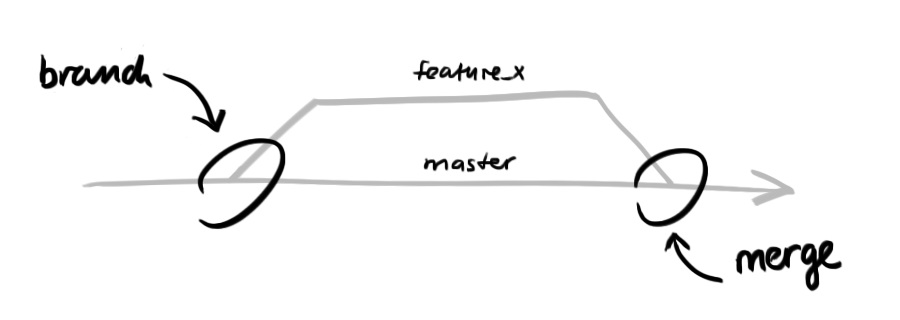
\includegraphics[width=0.6\linewidth]{branches}}

Lors d'un conflit, on se retrouvera avec des choses du genre suivant :

{\setstretch{1}
\begin{boxedverbatim}
$ git merge myBranchFromB
Auto-merging firstFile.txt
CONFLICT (content): Merge conflict in firstFile.txt
Automatic merge failed; fix conflicts and then commit the result.
$ cat firstFile.txt
This is the first line of my first file...
... and this is the second line
Now we add another line
 
Adding a fourth line
Adding a fifth line
modification from repoA
modifications from repoB
<<<<<<< HEAD
conflict from repoA
=======
conflict from repoB
>>>>>>> myBranchFromB
- See more at: ....
\end{boxedverbatim}
}

%\newpage

Pour le résoudre, il n'y a pas d'autre choix que de le faire à la main ! Eh oui \emph{git} ne pourra pas deviner qui a raison et tort, ou si les deux sont justes/fausses ! On va donc éditer la zone entre les chevrons avec notre éditeur préféré.

\newpage 
\section{Nenufaar}
{\setstretch{1.2}
Dans cette partie, on va voir comment on peut utiliser \emph{git} dans le cadre du développement de Nenufaar. On va configurer le compte \emph{bitbucket} puis voir un exemple de dév. L'exemple n'est pas à effectuer, mais il permet de comprendre comment utiliser \emph{git} dans ce contexte.

\subsection{Bitbucket}

\emph{Bitbucket} est un service d'hébergement et de gestion de développement logiciel. En premier lieu crée votre compte sur \emph{\href{https://bitbucket.org}{https://bitbucket.org}}. Ensuite, envoyez moi vos identifiants pour que je puisse vous rajouter au projet. Vous recevrez un lien par mail pour vous ajouter au projet. Et voilà, vous êtes ajouté à l'équipe IURC ! Vous pouvez maintenant cloner le projet Nenufaar !

\subsubsection{Configurer la connexion SSH}

\paragraph*{SSH : kézako ?} SSH signifie \emph{Secure SHell}. C'est un protocole de connexion sécurisé entre deux machines. Cela permet donc de communiquer, d'échanger des données, entre un client et un serveur par chiffrement, ici nous utilisons le chiffrement RSA (du nom de ses inventeurs Rivest, Shamir, Adleman). En effet, \emph{Bitbucket} nous offre la possibilité de relier notre machine à notre compte à l'aide de ce protocole. 

\paragraph{Générer la clé RSA} Aller dans votre terminal préféré et lancer la commande suivante pour savoir si vous avez une clé rsa :
}

{\setstretch{1}
\begin{boxedverbatim}
$ more ~/.ssh/id_rsa.pub
ssh-rsa sdfZTZETZGgzgze45...64564egdGDFGd9_90DSGF user@computer
\end{boxedverbatim}
}

Si vous obtenez un truc du genre, vous avez une clé RSA, sinon on doit générer notre clé rsa à l'aide des commandes suivantes :

{\setstretch{1}
\begin{boxedverbatim}
$ ssh-keygen -t rsa
Generating public/private rsa key pair.
Enter file in which to save the key (/home/user/.ssh/id_rsa):
Enter passphrase (empty for no passphrase): 
Your identification has been saved in /home/user/.ssh/id_rsa.
Your public key has been saved in /home/user/.ssh/id_rsa.pub.
The key fingerprint is:
SHA256:zPZxXxrdNDGvTEA20wHAn0FFiV34zYyFDha964gW5Ow user@computer
The key's randomart image is:
+---[RSA 2048]----+
|     .+o+BOB+o   |
|      o+o=oo=+o  |
|       o+.o+.B+..|
|      .= .+0=ooo.|
|      .ES . + o .|
|       . + o +   |
|            .    |
+----[SHA256]-----+
\end{boxedverbatim}
}

Et voilà votre clé RSA toute belle ! On la copie et on passe au niveau suivant !

\vspace{1cm}

\begin{minipage}{0.25\linewidth}
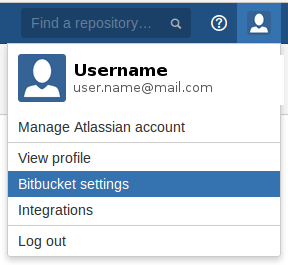
\includegraphics[width=\linewidth]{bitbucket1}
\end{minipage}\hfill
\begin{minipage}{0.75\linewidth}
\textbf{Relier son compte à sa clé} Pour cela on commence par se connecter à son compte \emph{Bitbucket}. Ensuite rendez-vous dans les paramètre du compte \emph{avatar} -> Bitbucket settings.
\end{minipage}

\vspace{1cm}

\begin{minipage}{0.25\linewidth}
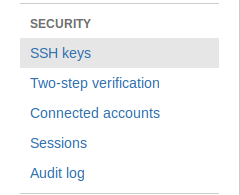
\includegraphics[width=\linewidth]{bitbucket2}
\end{minipage}\hfill
\begin{minipage}{0.75\linewidth}
Maintenant dans le menu de gauche cliquer sur \emph{SECURITY} -> SSH keys
\end{minipage}

Vous arriverez sur un panneau qui vous propose d'ajouter une nouvelle clé. Cliquer sur \emph{Add key}. Une fenêtre s'ouvre et vous propose d'ajouter une clé SSH. Copier le contenu du fichier \emph{\textasciitilde /.ssh/id\_rsa.pub}. Vous pouvez rajouter un label pour savoir quelle clé correspond à quelle machine.

\centerline{
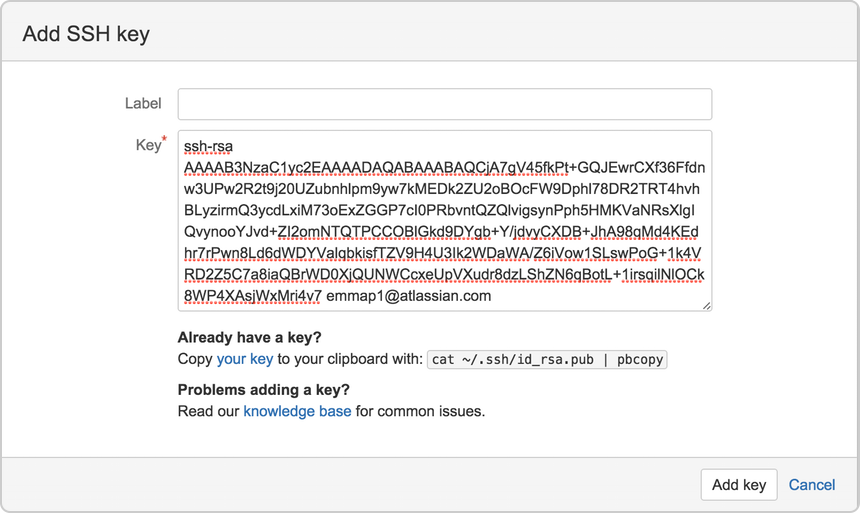
\includegraphics[width=0.6\linewidth]{add_ssh_key}}

\subsection{Un exemple concret}

C'est cool ça ! Si l'on prenait un cas concret maintenant ! On va supposer que je suis chargé d'intégrer une nouvelle fonction à Nenufaar (par exemple : intégrer un caller somatique). Chaque étape se déroulera comme suit :
\begin{itemize}
\item[$\bullet$] un paragraphe qui décrit ce que l'on fait ;
\item[$\bullet$] les lignes de codes correspondantes ;
\item[$\bullet$] un graphique de l'avancement du projet.
\end{itemize}

\subsubsection{Le début}

La première chose à faire quand on intègre un projet c'est de le cloner. Ensuite, on peut directement, ou non, avoir des tâches à effectuer. Quelques jours après avoir cloné Nenufaar, une nouvelle version est sortie. Nenufaar est passé de la version 0 à la version 1. Je dois donc mettre à jour ma copie.

\vspace{1cm}

{\setstretch{1}
\begin{boxedverbatim}
$ git clone git@bitbucket.org:iurc/nenufaar.git
Clonage dans 'nenufaar'...
remote: Counting objects: 14, done.
remote: Compressing objects: 100% (11/11), done.
remote: Total 14 (delta 5), reused 0 (delta 0)
Réception d'objets: 100% (14/14), 5.09 KiB | 0 bytes/s, fait.
Résolution des deltas: 100% (5/5), fait.
Vérification de la connectivité... fait.

$ git remote update 
Récupération de origin
remote: Counting objects: 3, done.
remote: Compressing objects: 100% (3/3), done.
remote: Total 3 (delta 1), reused 0 (delta 0)
Dépaquetage des objets: 100% (3/3), fait.
Depuis bitbucket.org:iurc/nenufaar
   654a020..4e3b679  master     -> origin/master
   
$ git pull
Mise à jour 654a020..4e3b679
Fast-forward
 README.md | 4 ++--
 1 file changed, 2 insertions(+), 2 deletions(-)
\end{boxedverbatim}
}

\vspace{1cm}

\includegraphics[scale=0.4]{flow1}

\newpage

\subsubsection{Développement}

Je vais maintenant m'attaquer au développement afin d'intégrer un variant caller somatic. La première chose à faire et de créer une branche destinée à l'ajout de cette fonctionnalité. Je fais mes dév tranquilles en faisant des commit régulièrement. Et je \emph{push} mes modifications.

\vspace{1cm}

{\setstretch{1}
\begin{boxedverbatim}
$ git checkout -b DEV_caller_somatique
Basculement sur la nouvelle branche 'DEV_caller_somatique'

$ vim README.md

$ git commit README.md -m "add variant caller"
[DEV_caller_somatique 134853e] add variant caller
 1 file changed, 2 insertions(+), 2 deletions(-)
 
$ git push origin DEV_caller_somatiqueDécompte des objets: 3, fait.
Delta compression using up to 8 threads.
Compression des objets: 100% (3/3), fait.
Écriture des objets: 100% (3/3), 349 bytes | 0 bytes/s, fait.
Total 3 (delta 1), reused 0 (delta 0)
remote: 
remote: Create pull request for DEV_caller_somatique:
remote:   https://bitbucket.org/iurc/nenufaar/pull-requests
/new?source=DEV_caller_somatique&t=1
remote: 
To git@bitbucket.org:iurc/nenufaar.git
 * [new branch]      DEV_caller_somatique -> DEV_caller_somatique
\end{boxedverbatim}
}

\vspace{1cm}

\includegraphics[scale=0.4]{flow2}

\newpage

\subsubsection{Bugfix}

Je reçois un coup de téléphone de David, parti en conférence à New-York. Il m'explique alors qu'un utilisateur de Nenufaar a remarqué un bug (ou bogue en français). Il faut le corriger en urgence et il n'a pas le temps de le faire (jetlag, conférence, champagne tout ça quoi...), je dois donc le corriger. Je commence par créer une branche portant un numéro de bug par exemple (bugfix29). Et je m'attelle à la correction du Bug.

\vspace{1cm}

{\setstretch{1}
\begin{boxedverbatim}
$ git checkout master
$ git checkout -b bugfix29
Basculement sur la nouvelle branche 'bugfix29'

$ vim README.md

$ git commit README.md -m "fix bug"
[bugfix29 fe98406] fix bug
 1 file changed, 2 insertions(+), 2 deletions(-)

$ git push origin bugfix29
Décompte des objets: 3, fait.
Delta compression using up to 8 threads.
Compression des objets: 100% (3/3), fait.
Écriture des objets: 100% (3/3), 335 bytes | 0 bytes/s, fait.
Total 3 (delta 1), reused 0 (delta 0)
remote: 
remote: Create pull request for bugfix29:
remote:   https://bitbucket.org/iurc/nenufaar/pull-requests
/new?source=bugfix29&t=1
remote: 
To git@bitbucket.org:iurc/nenufaar.git
 * [new branch]      bugfix29 -> bugfix29
\end{boxedverbatim}
}

\vspace{1cm}

\includegraphics[scale=0.4]{flow3}

\newpage

\subsubsection{Relier au master}

Après avoir corrigé le bug, je peux fusionner la branche contenant le \emph{bugfix} avec la branche master. Puis supprimer la branche correspondant à la suppression du bug. Enfin, j'envoie les modifications sur le serveur.

\vspace{1cm}

{\setstretch{1}
\begin{boxedverbatim}
$ git checkout master
Basculement sur la branche 'master'
Votre branche est à jour avec 'origin/master'.

$ git merge bugfix29 
Mise à jour 4e3b679..fe98406
Fast-forward
 README.md | 4 ++--
 1 file changed, 2 insertions(+), 2 deletions(-)

$ git branch -d bugfix29
Branche bufix29 supprimée (précédemment fe98406).

$ git push
Total 0 (delta 0), reused 0 (delta 0)
To git@bitbucket.org:iurc/nenufaar.git
   4e3b679..fe98406  master -> master
\end{boxedverbatim}
}

\vspace{1cm}

\includegraphics[scale=0.4]{flow4}

\newpage

\subsubsection{Mise à jour de la \emph{feature}}

Je me replace maintenant au niveau de la branche de développement de la prochaine \emph{feature} sur laquelle je travaille actuellement. Il suffit que je fusionne la branche de développement avec la branche \emph{master} pour avoir la correction du bug.

\vspace{1cm}

{\setstretch{1}
\begin{boxedverbatim}
$ git checkout DEV_caller_somatique 
Basculement sur la branche 'DEV_caller_somatique'

$ git merge master 
Fusion automatique de README.md
Merge made by the 'recursive' strategy.
 README.md | 2 +-
 1 file changed, 1 insertion(+), 1 deletion(-)
\end{boxedverbatim}
}

\vspace{1cm}

\includegraphics[scale=0.4]{flow5}

\newpage

\subsubsection{Fin de développement de la \emph{feature}}

Après avoir finit de développer ma \emph{feature} je peux l'intégrer dans la branche \emph{master}. J'envoie mes modifications et c'est fini !

\vspace{1cm}

{\setstretch{1}
\begin{boxedverbatim}
$ git checkout master 
Basculement sur la branche 'master'
Votre branche est à jour avec 'origin/master'.

$ git merge DEV_caller_somatique 
Mise à jour fe98406..3ea1853
Fast-forward
 README.md | 2 +-
 1 file changed, 1 insertion(+), 1 deletion(-)
 
 $ git branch -d DEV_caller_somatique 
Branche DEV_caller_somatique supprimée (précédemment 3ea1853).

$ git push
Décompte des objets: 3, fait.
Delta compression using up to 8 threads.
Compression des objets: 100% (3/3), fait.
Écriture des objets: 100% (3/3), 398 bytes | 0 bytes/s, fait.
Total 3 (delta 1), reused 0 (delta 0)
To git@bitbucket.org:iurc/nenufaar.git
   fe98406..3ea1853  master -> master
\end{boxedverbatim}
}

\vspace{1cm}


\includegraphics[scale=0.4]{flow6}

\newpage



% \subsubsection{Travailler sur \emph{bitbucket}}

% Maintenant on va compliquer un peu les choses avec le travail à plusieurs. Ici on va voir l'application sur \emph{bitbucket}. \emph{Bitbucket} est un service d'hébergement et de gestion de développement logiciel.

% \paragraph{Créer son compte} Aller sur \emph{\href{https://bitbucket.org}{https://bitbucket.org}}

% %\subsubsubsection{Relier son compte de façon sécurisé}





% \section{Seconde partie}

% \subsection{Expérience}

% \subsection{Observations}

% \subsection{Conclusion}

\section{Un peu plus loin}

Voici quelques liens utiles pour aller plus loin et qui m'ont servi à rédiger ce petit cours :
\begin{itemize}
\item \href{http://bioinfo-fr.net/git-premiers-pas}{bioinfo-fr.net/git-premiers-pas}
\item \href{https://git-scm.com/doc}{git-scm.com/doc}
\item \href{http://www.slideshare.net/shengwen1997/brief-tutorial-on-git}{www.slideshare.net/shengwen1997/brief-tutorial-on-git}
\item \href{http://rogerdudler.github.io/git-guide/index.fr.html}{rogerdudler.github.io/git-guide/index.fr.html}
\item \href{https://www.git-tower.com}{www.git-tower.com}
\item \href{http://formation-debian.via.ecp.fr/ssh.html}{formation-debian.via.ecp.fr/ssh.html}
\item \href{https://doc.ubuntu-fr.org/ssh}{doc.ubuntu-fr.org/ssh}
\end{itemize}

\newpage


\includepdf[pages={1}]{selection}
\end{document}